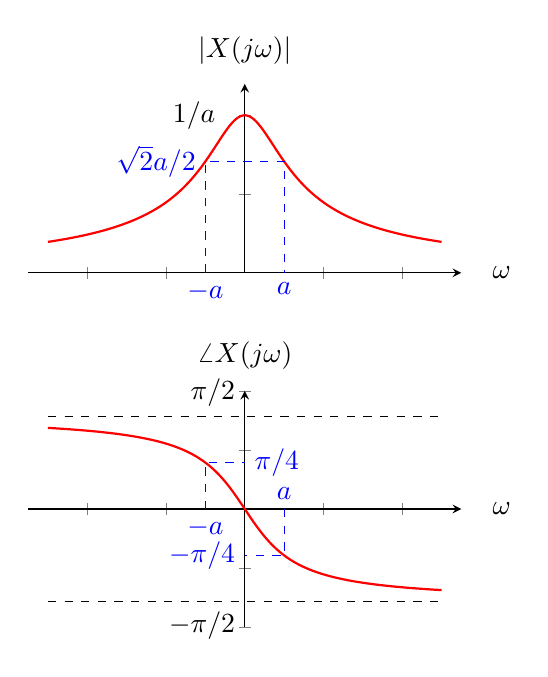
\begin{tikzpicture}[scale=1]
\begin{scope}	
    \begin{axis}[
		y=2cm,
		x=0.5cm,
		 clip=false,
		 xmin=-5.5,xmax=5.5,
		 xlabel= $\omega$,
		 ylabel={$|X(j\omega)|$},
		 ymin=0,ymax=1.2,
		 axis lines=middle,
         	%xtick={-5, -4, ..., 5},
		 %ytick={-1, 1},
		 yticklabels=\empty,
		 xticklabels=\empty,
		 every axis x label/.style={at={(ticklabel* cs:1.05)}, anchor=west,},
		every axis y label/.style={at={(ticklabel* cs:1.05)}, anchor=south,},
     ]
		%\addplot+[red, smooth, mark=none] table [x={n}, y={xn}] {periodic_square_fs_samples_of_envilope_gen.dat};
		\addplot [red, thick, domain=-5:5, samples=200] plot{1/sqrt(x*x + 1))};
		\node at (axis cs:-0.5, 1) [anchor=east] { $1/a$ };
		\draw[dashed, blue] (axis cs:-1, 0) node[anchor=north] { $-a$} -- (axis cs:-1, 0.707) node[anchor=east] { $\sqrt{2} a/2$} --  (axis cs:1, 0.707)  --  (axis cs:1, 0) node[anchor=north] { $a$} ;
    \end{axis}
\end{scope}

\begin{scope}[yshift=-4.5cm]	
    \begin{axis}[
		y=0.75cm,
		x=0.5cm,
		 clip=false,
		 xmin=-5.5,xmax=5.5,
		 xlabel= $\omega$,
		 ylabel={$\angle X(j\omega)$},
		 ymin=-2,ymax=2,
		 axis lines=middle,
         	%xtick={-5, -4, ..., 5},
		 %ytick={-1, 1},
		 yticklabels=\empty,
		 xticklabels=\empty,
		 every axis x label/.style={at={(ticklabel* cs:1.05)}, anchor=west,},
		every axis y label/.style={at={(ticklabel* cs:1.05)}, anchor=south,},
     ]
		%\addplot+[red, smooth, mark=none] table [x={n}, y={xn}] {periodic_square_fs_samples_of_envilope_gen.dat};
		\addplot [red, thick, domain=-5:5, samples=200] plot{-rad(atan(x))};
		\draw[dashed, blue] (axis cs:1, 0) node[anchor=south] { $a$} -- (axis cs:1, -pi/4)  -- (axis cs:0, -pi/4) node[anchor=east] { $-\pi/4$} ;
		\draw[dashed, blue] (axis cs:-1, 0) node[anchor=north] { $-a$} -- (axis cs:-1, pi/4)  -- (axis cs:0, pi/4) node[anchor=west] { $\pi/4$} ;
		\draw[dashed, black] (axis cs:-5, pi/2) --   (axis cs:5, pi/2) node[midway, anchor=south east] {$\pi/2$} ;
		\draw[dashed, black] (axis cs:-5, -pi/2) --   (axis cs:5, -pi/2) node[midway, anchor=north east] {$-\pi/2$} ;
   \end{axis}
\end{scope}
\end{tikzpicture} 